% give me a starting template for a latex report with a table of contents 2 chapters long

\documentclass[12pt]{article}

\title{Avance 1 - Proyecto Base de Datos I}
\author{}

\usepackage{graphicx}
\usepackage{listings}
\usepackage{color}
\usepackage{amsmath}
\usepackage{hyperref}


\begin{document}

\maketitle

\tableofcontents

\newpage

\section{Requisitos}

\subsection{Introducci\'on}

En este proyecto se desea desarrollar una base de datos para una tienda de autos que se dedica a la compra de vehículos de otras empresas, nuevos y seminuevos, para revenderlos al público. La tienda se basa en tiendas como <nombre de tienda> y tiene como objetivo ofrecer vehículos asequibles para el peruano promedio. Debido a la naturaleza de constante rotación de mercancía es necesario modelar una base de datos robusta que permita la entrada de los vehículos adquiridos y la fácil y eficiente consulta de aquellos que están en stock. 

\subsection{Descripci\'on general del problema/organizaci\'on/empresa}

La necesidad de vehículos motorizados es importante en la ciudad de Lima, ya que el transporte público no está muy desarrollado. La tienda de autos busca solucionar esta necesidad ofreciendo vehículos nuevos y seminuevos a precios accesibles, al obtenerlos en suministros de gran cantidad directamente de diversas empresas distribuidoras de vehiculos, o que venden sus flotas usadas de trabajo.

El problema recae en el monitoreo y manejo de la información de esta gran cantidad de vehiculos que rota constantemente en el stock de la tienda. Al usar métodos tradicionales como registros a mano, se requiere mucho tiempo al realizar la compra y venta de vehículos, es difícil para el cliente saber qué tiene la tienda a la venta, existe la posibilidad de error en la lectura y escritura, y se pierde la posibilidad de análisis estadístico de las ventas de la empresa (para obtener un mayor márgen de ganancia/más ventas).

\subsection{Necesidad/usos de la base de datos}

La base de datos es necesaria para llevar un control de los vehículos que se compran, se venden y los que se encuentran en inventario, así como también para llevar un registro de los clientes, los asesores de venta y los proveedores.

\subsection{¿Cómo resuelve el problema de hoy?}

La tienda actualmente lleva un registro manual de los vehículos, los clientes y las ventas, lo cual es un proceso lento y propenso a errores. La base de datos ayudará a mejorar el proceso de registro y seguimiento de los vehículos, clientes y ventas. La implementación de la base de datos en la tienda es la solución.

\subsubsection{¿Cómo se almacenan/procesan los datos hoy?}

Actualmente los datos se almacenan en archivos físicos (papel) y en hojas de cálculo en línea (Excel). No hay una base de datos centralizada y el proceso de registro de los vehículos, clientes y ventas se hace manualmente. La consulta de datos se hace igualmente de forma manual.

\subsubsection{Flujo de datos}

El flujo de datos actual comienza con el suministro de vehículos realizado por parte de los proveedores, seguido de la recepción de los vehículos por parte de la tienda. En caso de que el modelo o motor del vehículo no estén registrados, se tienen que añadir previamente a las tablas correspondientes. A continuación, los vehículos son agregados al inventario de la tienda. Los clientes consultan el inventario y realizan compras, supervisadas por los asesores de ventas. Por último, la orden de compra es registrada y el vehiculo deja de ser mostrado en el inventario de la tienda. Los clientes pueden consultar el historial de compras que han realizado ellos.

\subsection{Descripci\'on detallada del sistema}

\subsubsection{Objetivos de información actuales}

Los objetivos de información actuales son llevar un control de los vehículos en inventario (tanto en la compra y venta de estos), permitir a los clientes consultar los vehículos disponibles, llevar control de las compras que remueven (u ocultan) a los vehículos de la base de datos.

\subsubsection{Caracter\'isticas y funcionalidades esperadas}

Se espera que la base de datos permita llevar un registro de los vehículos en inventario, de los clientes y de las ventas realizadas. También se espera que permita generar reportes y estadísticas sobre el inventario, las ventas y los clientes.

\subsubsection{Tipos de usuarios existentes/necesarios}

Los tipos de usuarios necesarios son los asesores de ventas, los clientes y los proveedores. Se espera que el proveedor brinde la información requerida de cada vehículo suministrado, la cual será incorporada en la base de datos. Así se elimina la necesidad de añadir manualmente con un administrador.

\subsubsection{Tipos de consulta, actualizaciones}

Los tipos de consulta y actualización que se esperan por parte de los clientes son: Consulta del stock (vehículos),  consulta de las compras realizadas. Actualización (Eliminar/ocultar) la lista de vehículos al realizar la compra, registro de la compra.

Los proveedores registran la lista de vehículos al realizar el suministro. Igualmente registran en motor y modelo cuando se añaden vehículos con estos no presentes.

son consultas de inventario, consultas de clientes y consultas de ventas realizadas. Las actualizaciones que se esperan son actualizaciones de inventario, actualizaciones de clientes y actualizaciones de ventas realizadas.

\begin{tabular}{|l|l|l|}
\hline
\textbf{Tabla} & \textbf{Tamaño de atributos} & \textbf{Total} \\ \hline
Cliente       &                            & 10             \\ \hline
Asesor        & 10                           & 10             \\ \hline
Proveedor     & 10                           & 10             \\ \hline
Empresa       & 10                           & 10             \\ \hline
Compra        & 10                           & 10             \\ \hline
Suministro    & 10                           & 10             \\ \hline
Vehículo      & 10                           & 10             \\ \hline
Motor         & 10                           & 10             \\ \hline
Modelo        & 10                           & 10             \\ \hline
\end{tabular}
\subsubsection{Tama\~no de la base de datos}

El tamaño de la base de datos es directamente proporcional al tamaño del negocio, así como la frecuencia de las ventas. El tamaño del negocion nos da una perspectiva de la cantidad de vehículos en stock por vez, y la frecuencia de las ventas nos da una perspectiva de la tasa de crecimiento de las tablas de clientes y compras.

En el caso de autoland, estimamos unas 40 ventas por mes, y aproximadamente 5000 ventas anuales. Esto nos da un estimado de una entrada de al menos 100 000 datos anuales, incluyendo la información de los suministros, los clientes, las compras, y las especificaciones de los vehículos.

\subsection{Objetivos del proyecto}



\subsection{Referencias del proyecto}

El proyecto se inspiró en tiendas de autos como Autoland, que tienen un gran stock de vehículos y que necesitan llevar un registro de los mismos, así como de los clientes y las ventas realizadas. Originalmente planeamos un portal en línea como neoauto donde se pueden comprar y vender vehículos, pero decidimos que una base de datos para una tienda funcionaría mejor.

\subsection{Eventualidades}

\subsubsection{Problemas que pudieran encontrarse en el proyecto}

Nuestro proyecto cuenta con las siguientes posibles problemas:

\begin{itemize}

\item No se incluye un sistema de autenticación de usuarios, por lo que no se puede distinguir entre los diferentes tipos de usuarios (clientes, asesores de ventas, proveedores) cuando se filtre por su llave única (DNI).

\item La base de datos no considera servicios de mantenimiento, ni de reparación de vehículos.

\item Se ha priorizado el entendimiento del modelo por encima de la eficiencia de las consultas, por lo que el tiempo de consultas puede no ser el ideal.



\end{itemize}


\subsubsection{Limites y alcances del proyecto}

\begin{itemize}

\item Alcances

Este proyecto tendrá un alcance a cualquier tienda con un modelo de negocio compatible dentro del país, y se espera que sea usada por una tienda de venta de vehículos como Autoland, la cual cuenta con sedes en diversos distritos de la ciudad de Lima Metropolitana.

\item Limites

Este proyecto no aplica para tiendas de venta de vehículos que no tengan un modelo de negocio compatible, como por ejemplo, tiendas de venta de vehículos de segunda mano que compran a personas naturales en vez de personas jurídicas (empresas). Tampoco considera negocios que lidien con extranjeros, sea al contratarlos como asesores, o al vender a clientes sin documento de identidad nacional (DNI).


\end{itemize}


\section{Modelo Entidad-Relaci\'on}

\subsection{Reglas sem\'anticas}

A continuación, las reglas semánticas que definen el fucionamiento de la base de datos.

\begin{itemize}
\item La tienda contrata asesores de ventas que se encargan de supervisar la venta de vehículos. Cuentan con DNI, RUC, Nombres, Apellidos y Salario.
\item La tienda contrata mecánicos que se encargan de inspeccionar los vehículos antes de su venta, así como realizar servicios de mantenimiento y reparación a los clientes. Cuentan con DNI, RUC, Nombres, Apellidos y Salario.
\item Los clientes se identifican con su DNI, Nombres y Apellidos. Para ser considerado cliente, debe haber realizado por lo menos una compra.
\item Los proveedores son los agentes que nos suministran de vehículos. Se identifican con su DNI. Cuentan con nombres, apellidos, y el RUC de la empresa en la que trabaja. Cada proveedor trabaja para una sola empresa, que se identifica con su razón social y RUC.
\item Los clientes pueden realizar múltiples compras (las compras dependen del cliente).
\item La compra de un vehículo debe ser atendida solo por un asesor de ventas, y se registra con un código numérico único, fecha, DNI del cliente, DNI del asesor y VIN del vehículo.
\item Cada compra corresponde a la adquisición de un solo vehículo.
\item Los proveedores realizan suministros. Para ser registrado como proveedor debe haber realizado mínimo un suministro a la tienda.
\item Cada suministro corresponde a un solo proveedor. Igualmente no existe sin éste.
\item Cada suministro añade uno o más vehículos al inventario de nuestra empresa.
\item Cada suministro se identifica con un código y el DNI de su proveedor. Además incluye fecha, y el importe total.
\item Tenemos vehículos cuyo identificador único es el número VIN.
\item Los vehículos cuentan con el color de pintura y precio de venta.
\item Los vehículos, si son usados, tienen kilometraje. Si son nuevos, este será 0.
\item Todos los vehículos cuentan con una transmisión.
\item La transmisión puede ser de 3 tipos: automática, manual o secuencial.
\item Los vehículos cuentan con un solo motor.
\item El motor se identifica por su código alfanumérico. Además, este tiene como atributos su marca, tipo de combustible, disposición, número de cilindros, cilindrada, y finalmente, la potencia.
\item Cada vehículo corresponde a exactamente un Modelo.
\item Todos los modelos se identifican por su ID numérico único, además tienen Marca, Nombre, Año y Precio Sugerido.
\item Hay 4 categorías de Modelo: Auto, camioneta, moto y camión.
\end{itemize}

\subsection{Modelo Entidad-Relaci\'on}

A continuación, el modelo entidad-relación que representa la base de datos:

\begin{figure}
\centering
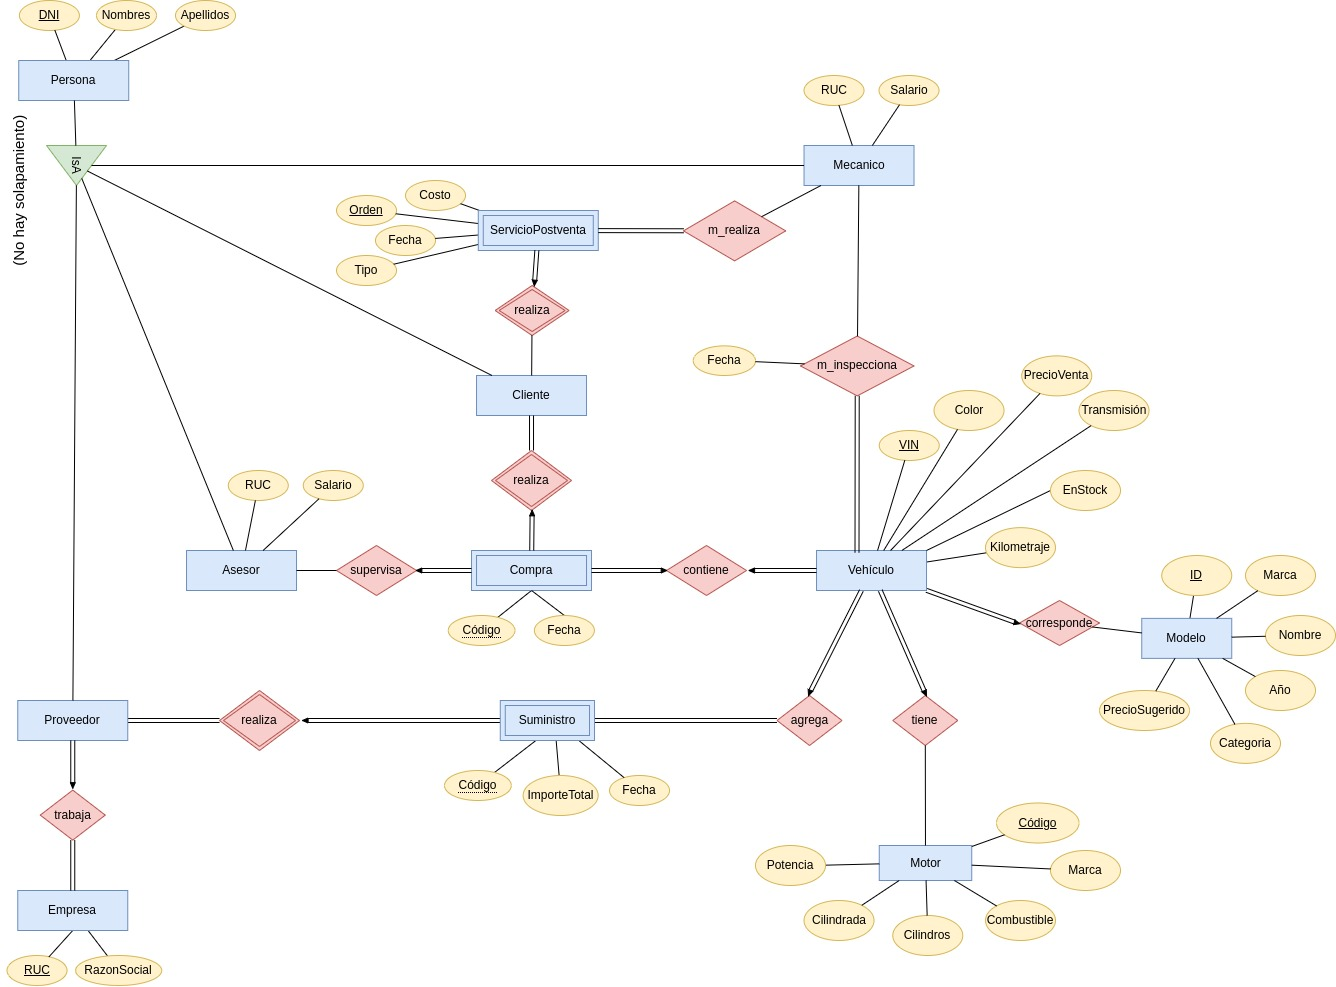
\includegraphics[width=0.8\textwidth]{ER.jpg}
\caption{Modelo Entidad-Relación}
\end{figure}

\subsection{Especificaciones y conseideraciones sobre el modelo}

\subsubsection{Entidad Persona}
\textbf{Especificaciones}

Clase padre de Cliente, Asesor, Mecánico y Proveedor. Contiene la información necesaria para identificarlos como sus Nombres y Apellidos, y su llave primaria es el DNI.
\textbf{Consideraciones}

Se usa el DNI como llave primaria por la posibilidad de homonimia y la facilidad que este provee como identificador único.

\subsubsection{Entidad Cliente}
\textbf{Especificaciones}

Contiene información específica del cliente, como su dirección, correo electrónico y teléfono, y su llave primaria es el DNI.
\textbf{Consideraciones}

Un cliente puede tener múltiples vehículos, por lo que se establece una relación entre las entidades Cliente y Vehículo.

\subsubsection{Entidad Asesor}
\textbf{Especificaciones}

Contiene información específica del asesor, como su número de empleado y fecha de contratación, y su llave primaria es el DNI.
\textbf{Consideraciones}

Un asesor puede atender a múltiples clientes y vehículos, por lo que se establece una relación entre las entidades Asesor, Cliente y Vehículo.

\subsubsection{Entidad Mecánico}
\textbf{Especificaciones}

Contiene información específica del mecánico, como su número de empleado y especialidad, y su llave primaria es el DNI.
\textbf{Consideraciones}

Un mecánico puede trabajar en múltiples servicios y vehículos, por lo que se establece una relación entre las entidades Mecánico, ServicioPostVenta y Vehículo.

\subsubsection{Entidad Proveedor}
\textbf{Especificaciones}

Contiene información específica del proveedor, como su dirección y número de contacto, y su llave primaria es su nombre.
\textbf{Consideraciones}

Un proveedor puede proveer múltiples suministros, por lo que se establece una relación entre las entidades Proveedor y Suministro.

\subsubsection{Entidad Empresa}
\textbf{Especificaciones}

Contiene información específica de la empresa, como su nombre y dirección, y su llave primaria es su nombre.
\textbf{Consideraciones}

Una empresa puede tener múltiples proveedores y empleados, por lo que se establece una relación entre las entidades Empresa, Proveedor y Persona.

\subsubsection{Entidad Suministro}
\textbf{Especificaciones}

Contiene información específica del suministro, como su nombre y precio, y su llave primaria es su nombre.
\textbf{Consideraciones}

Un suministro puede ser proporcionado por múltiples proveedores, por lo que se establece una relación entre las entidades Proveedor y Suministro.

\subsubsection{Entidad Compra}
\textbf{Especificaciones}

Contiene información específica de la compra, como su fecha y cantidad, y su llave primaria es un identificador único.
\textbf{Consideraciones}

Una compra puede incluir múltiples suministros y ser realizada por múltiples empleados, por lo que se establece una relación entre las entidades Compra, Suministro y Persona.

\subsubsection{Entidad Vehículo}
\textbf{Especificaciones}

Contiene información específica de cada vehículo que se ha tenido en stock, como su marca y modelo, y su llave primaria es su número de identificación.
\textbf{Consideraciones}



\subsubsection{Entidad Modelo}
\textbf{Especificaciones}

\textbf{Consideraciones}


\subsubsection{Entidad ServicioPostVenta}
\textbf{Especificaciones}

\textbf{Consideraciones}


\section{Modelo Relacional}

\subsection{Modelo Relacional}
\subsection{Especificaciones de transformaci\'on}

\subsubsection{Entidades}


\begin{tabular}{|c|c|}
\hline
Tabla & Asesor \\
\hline
Clave Primaria & \textbf{\underline{DNI}} \\
\hline
Clave Foránea & RUC \\
\hline
\end{tabular}


\begin{tabular}{|c|c|}
\hline
Tabla & Mecánico \\
\hline
Clave Primaria & \textbf{\underline{DNI}} \\
\hline
Clave Foránea & RUC \\
\hline
\end{tabular}


\begin{tabular}{|c|c|}
\hline
Tabla & Proveedor \\
\hline
Clave Primaria & \textbf{\underline{DNI}} \\
\hline
Clave Foránea & Empresa.RUC \\
\hline
\end{tabular}


\begin{tabular}{|c|c|}
\hline
Tabla & Empresa \\
\hline
Clave Primaria & \textbf{\underline{RUC}} \\
\hline
Clave Foránea & N/A \\
\hline
\end{tabular}



\begin{tabular}{|c|c|}
\hline
Tabla & Vehículo \\
\hline
Clave Primaria & \textbf{\underline{VIN}} \\
\hline
Clave Foránea & Motor.Código, Modelo.ID, Cliente.DNI \\
\hline
\end{tabular}


\begin{tabular}{|c|c|}
\hline
Tabla & Motor \\
\hline
Clave Primaria & \textbf{\underline{Código}} \\
\hline
Clave Foránea & N/A \\
\hline
\end{tabular}


\begin{tabular}{|c|c|}
\hline
Tabla & Modelo \\
\hline
Clave Primaria & \textbf{\underline{ID}} \\
\hline
Clave Foránea & N/A \\
\hline
\end{tabular}


\subsubsection{Entidades d\'ebiles}


\begin{tabular}{|c|c|}
\hline
Tabla & Compra \\
\hline
Clave Primaria & \textbf{\underline{Cliente.DNI}}, \textbf{\underline{Código}} \\
\hline
Clave Foránea & Asesor.DNI, Vehículo.VIN \\
\hline
\end{tabular}


\begin{tabular}{|c|c|}
\hline
Tabla & Suministro \\
\hline
Clave Primaria & \textbf{\underline{Proveedor.DNI}}, \textbf{\underline{Código}}, \textbf{\underline{Fecha}} \\
\hline
Clave Foránea & N/A \\
\hline
\end{tabular}


\begin{tabular}{|c|c|}
\hline
Tabla & ServicioPostventa \\
\hline
Clave Primaria & \textbf{\underline{Cliente.DNI}}, \textbf{\underline{Orden}}, \textbf{\underline{Fecha}} \\
\hline
Clave Foránea & N/A \\
\hline
\end{tabular}


\subsubsection{Entidades superclase/subclase}



\subsubsection{Relaciones binarias}

\begin{tabular}{|c|c|}
\hline
Tabla & m\_inspecciona \\
\hline
Clave Primaria & \textbf{\underline{Mecánico.DNI}}, \textbf{\underline{Vehículo.VIN}} \\
\hline
Clave Foránea & N/A \\
\hline
\end{tabular}

\subsubsection{Relaciones ternarias}

\subsection{Diccionario de datos}

\begin{table}[htbp]
    \begin{center}
    \begin{tabular}{|l|l|l|l|l|}
        \hline
        Nombre Campo & Tipo de dato & PK & FK & Descripción \\
        \hline
        DNI & VARCHAR(8) & X &  & Número de identificación del asesor \\
        Nombres & VARCHAR(50) &  &  & Nombres del asesor \\
        Apellidos & VARCHAR(50) &  &  & Apellidos del asesor \\
        RUC & VARCHAR(11) &  &  & Registro Único del Contribuyente del asesor \\
        Salario & FLOAT &  &  & Salario del asesor \\
        \hline
        \end{tabular}
        \caption{Tabla Asesor}
        \label{tab:tablas}
    \end{center}
\end{table}

\end{document}
